\subsection{High-level Architecture}
\label{sec:architecture}

\begin{figure*}[t]
	\centering
	\begin{subfigure}[t]{0.8\textwidth}
		%        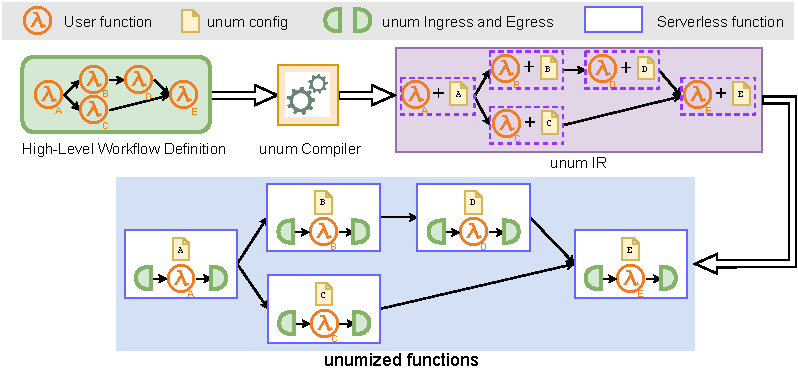
\includegraphics[width=\columnwidth]{figures/unum-arch-compile-time.pdf}
		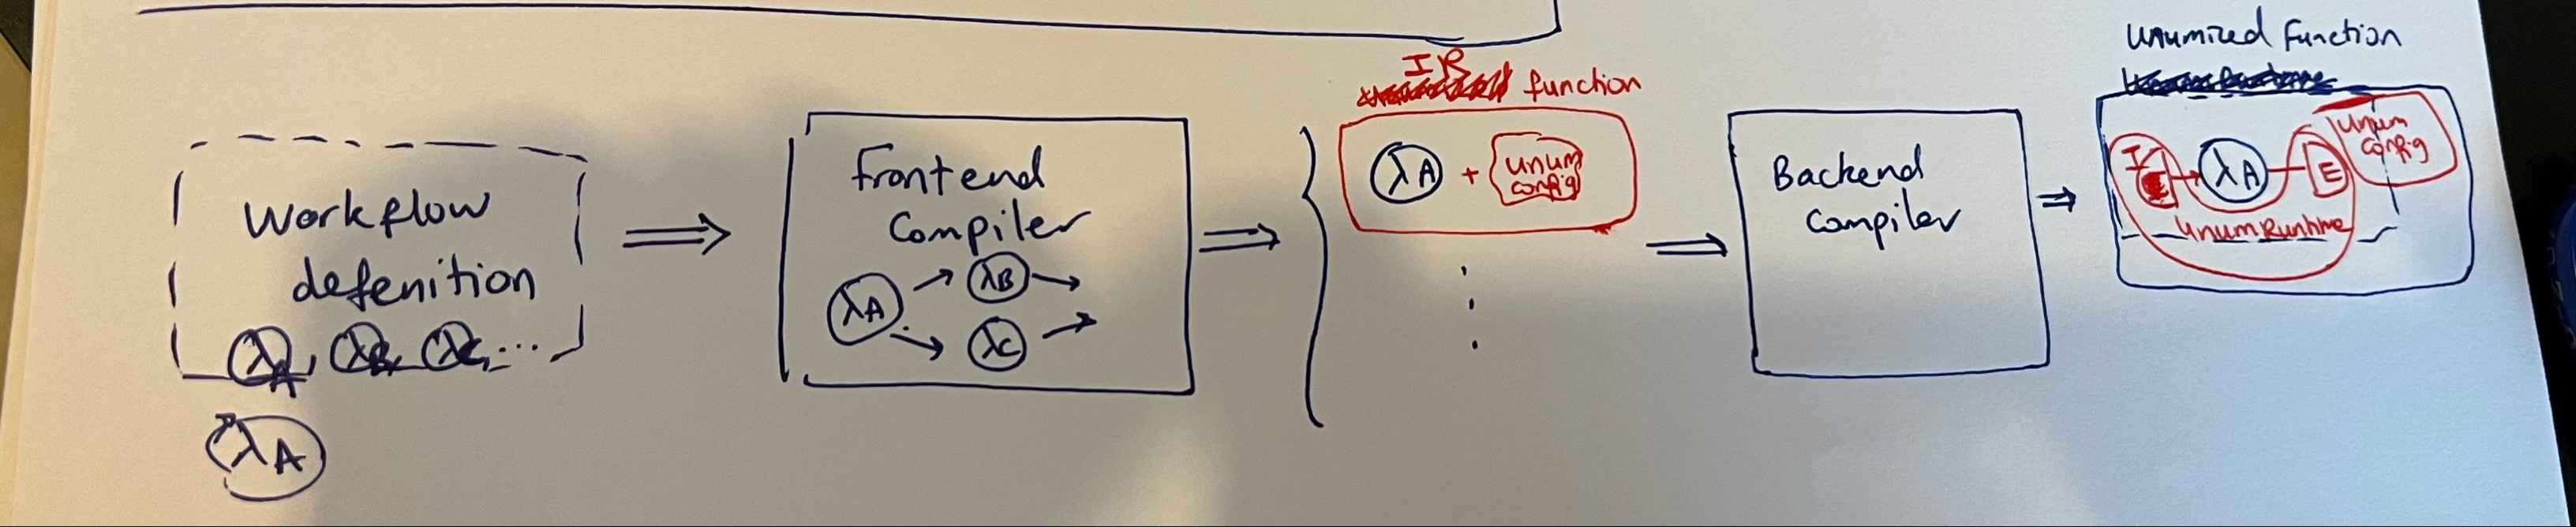
\includegraphics[width=\columnwidth]{figures/architecture.png}
		\caption{Stateful serverless computations form a directed graph. Nodes
			are user defined FaaS functions and ingress and egress ``gadgets'' that perform the necessary data movement, synchronization, and checkpointing between user functions.}
		\label{fig:arch:unum-compile-time}
		% unum injects gadgets to functions at compile time. But more
		% specifically, unum injects an encoding of gadgets at compile time.
		% The encoding expresses control-flow transitions just like what the
		% high-level workflow definition.
	\end{subfigure}
	\begin{subfigure}[b]{\columnwidth}
		\centering
		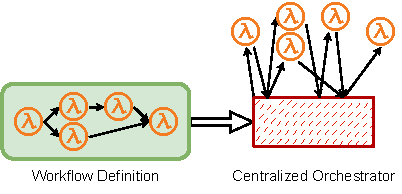
\includegraphics[width=0.8\columnwidth]{figures/unum-arch-centralized.pdf}
		\caption{A typical stateful serverless system drives workflow logic
			using a centralized controller that manages the computation's state-machine.}
		\label{fig:arch:centralized}
	\end{subfigure}
	\hfill
	\begin{subfigure}[b]{\columnwidth}
		\centering
		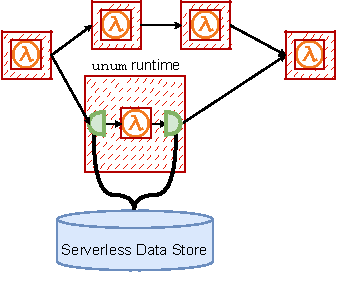
\includegraphics[width=.7\columnwidth]{figures/unum-arch-runtime.pdf}
		\caption{At runtime, all \name{} control logic is decentralized and runs within the Faas 
			functions executed on an unmodified serverless platform. For synchronization and checkpointing, \name{} relies exclusively on a
			standard datastore of choice, such as DynamoDB or Cosmos DB.}
		\label{fig:arch:unum-runtime}
	\end{subfigure}
	\caption{\name{} System Overview. Serverless computations form a directed
		graph that encode sequential and data dependencies between functions. Workflow
		orchestrators drive these graphs by centralizing control flow logic and
		interposing on all communication between functions. \name{},
		instead, decentralizes control flow logic among the functions with
		no need for a separate orchestration system.}
	\label{fig:arch}
\end{figure*}


Similar to other workflow systems~\cite{aws-step-functions, google-workflows,
	google-cloud-composer, gg-atc}, in \name{} users define their workflows using
a high-level description language that (directly or indirectly) expresses the
control-flow in the form of directed graphs  where nodes are serverless
functions and edges are control-flow transitions between functions. \name{'s} modular and extensible design supports integration with all commonly used high-level languages, e.g., Step functions representing workflows as state machines and Google
Workflows, Apache Airflow, Dask, representing workflows as DAGs\footnote{Our current implementation of \name{} is based on Step Functions.}.
%

Different from existing systems where a centralized orchestrator executes
the control-flow graph, \name{} partitions the control flow logic;  embeds the control flow alongside each individual function; and executes the functions in a distributed manner, with no centralized controller or additional services. Figure~\ref{fig:arch:unum-compile-time} shows the steps involved. First, the  \name{} compiler transforms the high-level workflow into a directed graph representation, e.g., converting the Step function state machines to a directed graph. Using this graph, the compiler outputs an platform agnostic intermediate representation (IR) represented as a set of IR functions, i.e, the user functions with the \name{} config embedded into it. the \name{} config includes the configuration on transition from the current function to the next function(s). Thus, instead of having a global view of the control-flow (in an orchestrator), the control-flow is distributed among functions such that each function just need to know where next to send the output. 

Next, the \name{} backend compiler converts the IR functions into \textit{unumized} functions, i.e., platform specific FaaS functions embedded with a \name{} runtime for that platform and the \name{} config. The user then deploys these unumized functions instead of its original functions. Upon execution, based on the \name{} config, the \name{} runtime  transparently, and in a decentralized manner, transitions data accordingly from one function to the next while also providing support for complex patterns such as fan-in. Additionally, the
runtime implements a checkpointing mechanism that ensures exactly-once
semantics (Section \shadi{?}).

This two step process in \name{} with the IR representation, enables portability to different function platforms (e.g., AWS Lambda or Azure Functions), and compatibility to different high-level languages as long as they can be compiled to a directed graph. Our current implementation is based on Step Functions as the API and AWS Lambda as the backend.


In this section, we first describe the transition patterns \name{} supports (Section~\ref{sec:transition-patterns}) and how these are executed in a decentralized manner (Section~\ref{sec:transition-execution}). Then, we describe the how we capture these patterns in our platform-agnostic IR representation (Section~\ref{sec:ir}). Finally, we describe how \name{} provides \shadi{....? describe the last sub sections.}. 


